\chapter{BCJ分子的构造}
本章是本论文的核心结论,首先介绍BCJ对偶,然后简述了从纯旋量形式出发如何得到SYM树级振幅以及任意点无质量态超弦盘面振幅公式。最后介绍了如何由此构造出树级SYM理论的BCJ分子。本章是充满技术性的章节,不少证明相当复杂,文中只给出了一些梗概,详细推导过程请见本文所引用文献。
\section{色-运动学对偶}
规范理论的振幅或是其圈图被积函数总能用三顶点图$\Gamma_n$求和表示:
\begin{equation}
	\label{eq:6.1}
	\mathcal{A}_n=\sum_{i\in\Gamma_n}\frac{c_iN_i}{D_i}
\end{equation}
三顶点图这一要求可以从规范理论振幅色因子都是一些结构常数$f^{abc}$的乘积,而这正好可以用三顶点图表示,这构成求和项中的$c_i$,$D_i$则是三顶点图结构给出的传播子,比如图\ref{fig:6.1}。

\begin{figure}[htbp]
	\centering
	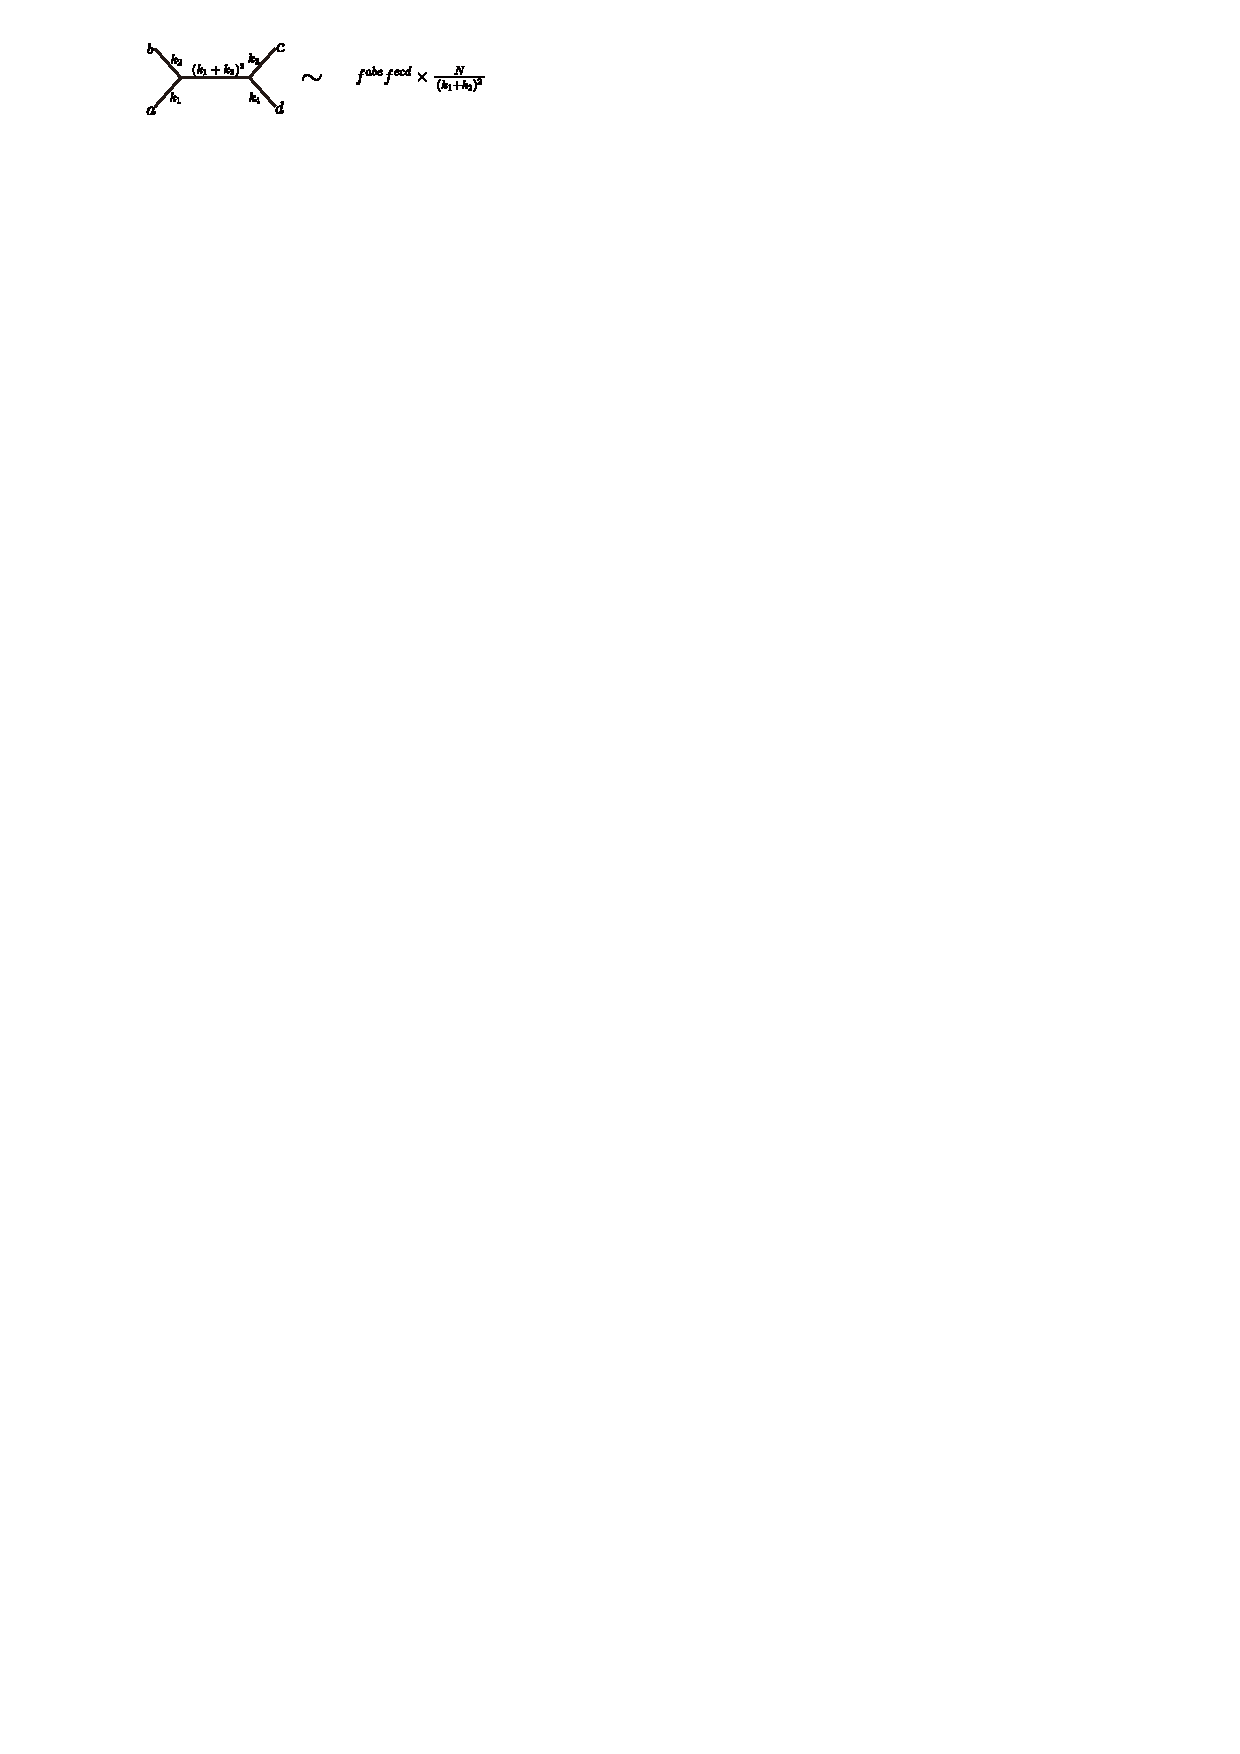
\includegraphics[width=0.8\linewidth]{figs/fig8.pdf}
	\caption{三顶点图“费曼”规则}
	\label{fig:6.1}
\end{figure}

众所周知,Yang-Mills理论费曼规则中不只有三顶角,还有四顶角,乍看之下似乎\ref{eq:6.1}有很大的漏洞。但实际上$\Gamma_n$不应该理解为费曼图,而只是组合学上对振幅的一种编码。但是这种编码的存在性又可以从费曼图本身看出来,比如费曼图四顶角可以用下面的一种方式约化为三顶角:
\begin{equation}
	\parbox[c]{\linewidth}{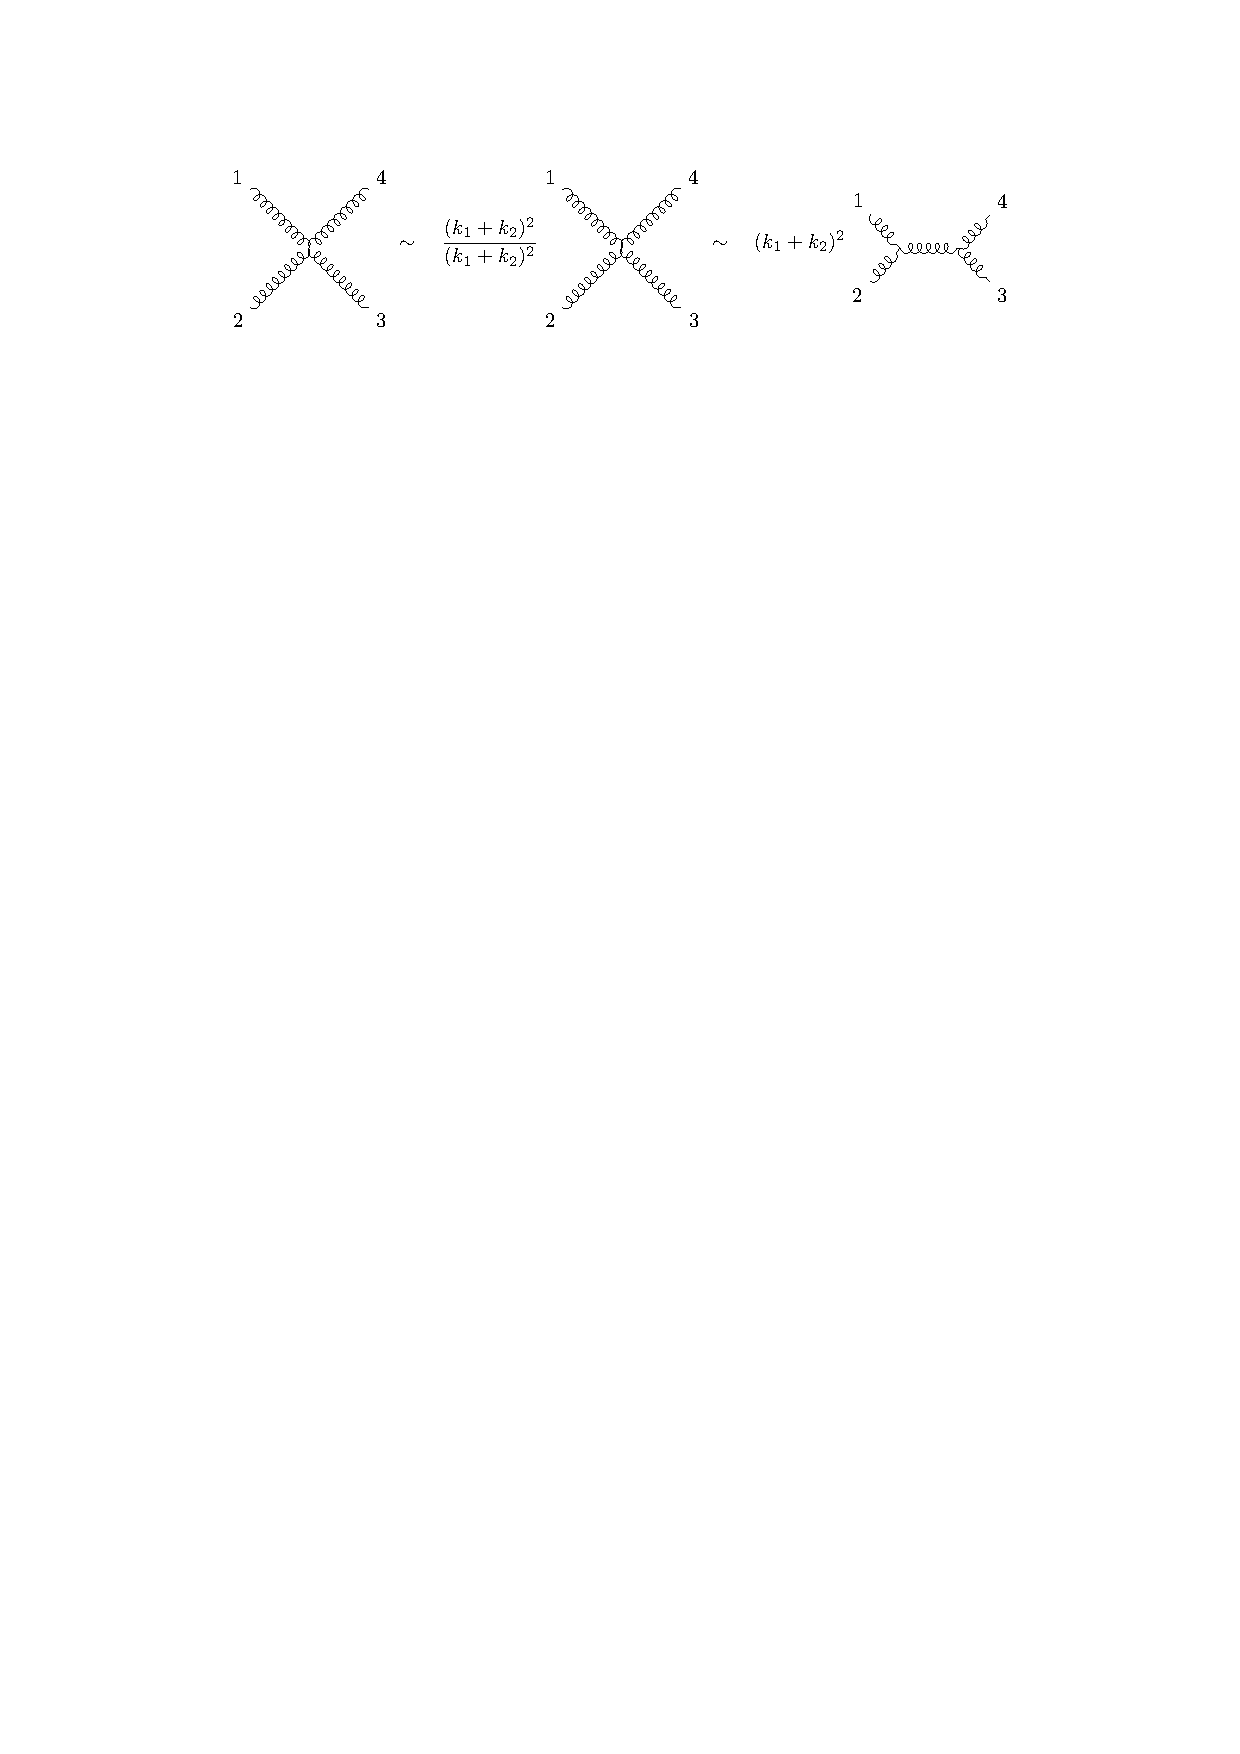
\includegraphics[width=\linewidth]{figs/eq_feyn.pdf}}
\end{equation}
显然,这种编码不是唯一的,但至少存在。结构常数满足如下的Jacobi恒等式:
\begin{equation}
	f^{abe}f^{ecd}+f^{bce}f^{ead}+f^{cae}f^{ebd}=0
\end{equation}
\begin{figure}[htbp]
	\centering
	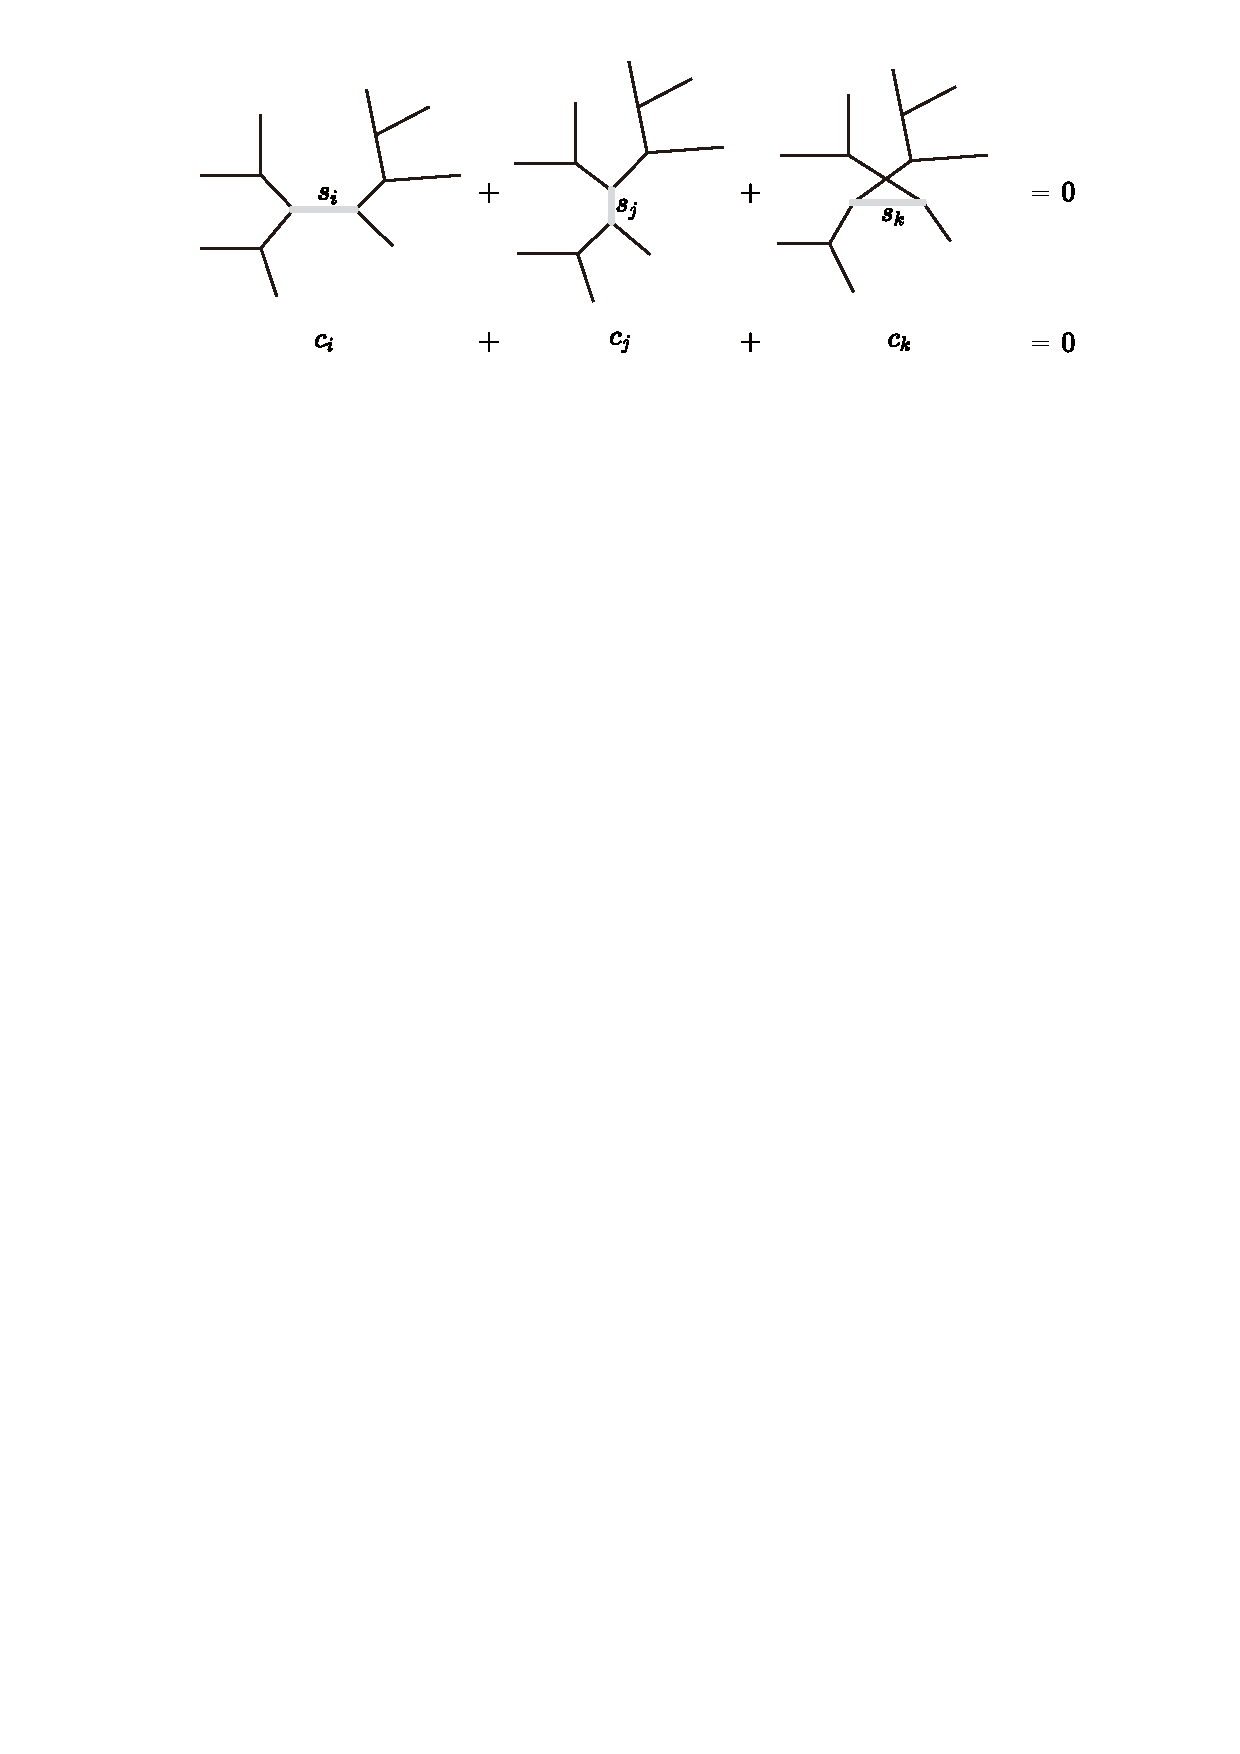
\includegraphics[width=0.95\linewidth]{figs/fig9.pdf}
	\caption{Jacobi恒等式}
	\label{fig:6.2}
\end{figure}
如图\ref{fig:6.2},这意味着三类图的色因子$c$之间的关系。同理$f^{abc}=-f^{acb}$也给出图上的关系。Bern-Carrasco-Johanson猜想存在$\{N_i\}$满足\ref{eq:6.1}而且满足和$\{c_i\}$同样的李代数结构\cite{Bern:2008qj}。也就是说对于任意$i,j,k\in\Gamma_n$:
\begin{equation}
\begin{aligned}
		c_i=-c_j\quad&\Leftrightarrow\quad N_i=-N_j\\
	c_i+c_j+c_k=0\quad&\Leftrightarrow\quad N_i+N_j+N_k=0
\end{aligned}
\end{equation}
这样的$\{N_i\}$称为BCJ分子,这个猜想也被称为色-运动学对偶。而且不难发现BCJ分子的选取不是唯一的,我们总是可以选取任意一个函数$\Delta$做如下变换得到新的BCJ分子:
\begin{equation}
	\label{eq:6.5}
	N_i\to N_i+s_i\Delta,\quad N_j\to N_j+s_j\Delta,\quad N_k\to N_k+s_k\Delta
\end{equation}
这里$s_i$,$s_j$和$s_k$是三幅图各自特有的传播子极点。对于后面要讨论的树图选取$[\lambda^a,\lambda^b] = f^{abc}\lambda^c$以及$\tr [\lambda^a,\lambda^b]=\delta^{ab}$的归一化约定,色基和迹基有如下关系:
\begin{equation}
	\label{eq:6.6}
	f^{a_1a_2x_1}f^{x_1a_3x_2}\cdots f^{x_{n-3}a_{n-1}a_n}=\operatorname{tr}\left(\lambda^{a_1}\left[\lambda^{a_2},[\lambda^{a_3},\ldots,[\lambda^{a_{n-1}},\lambda^{a_n}]\ldots]\right]\right)
\end{equation}
显然$\ref{eq:6.1}$给出如下的色序振幅:
\begin{equation}
	A_n(P)=\sum_{i\in\Gamma_n}\frac{N_i}{D_i}c_i\mid_{\tr (\lambda^P)}
\end{equation}
其中$c_i\mid_{\tr (\lambda^P)}\in\{0,\pm1\}$表示$c_i$中$\tr (\lambda^P)$前的符号。在后面对树图的讨论中,Del Duca–Dixon–Maltoni 基底是十分有用的\footnote{DelDuca:1999rs}:
\begin{equation}
	\label{eq:6.9}
	\mathcal{A}_n = \sum_{\sigma \in S_{n-2}} f^{a_1 a_{\sigma_1} b_1} f^{b_1 a_{\sigma_2} b_2} \cdots f^{b_{n-3} a_{\sigma_{n-2}} a_n} A_n(1, \sigma_1, \sigma_2, \ldots, \sigma_{n-2}, n)
\end{equation}
原本色运动学分离给出迹基底下的展开:
\begin{equation}
	\label{eq:6.10}
	\mathcal{A}_n=\sum_{\sigma\in S_{n-1}}\tr (\lambda^{a_{\sigma_1}}\lambda^{a_{\sigma_2}}\cdots \lambda^{a_{\sigma_{n-1}}}\lambda^{a_n})A_n(\sigma_1,\sigma_2,\ldots,\sigma_{n-1},n)
\end{equation}
但这些色序振幅之间仍有K-K关系\ref{KK},另外色基和迹基之间有关系\ref{eq:6.6},联合起来便可以从\ref{eq:6.10}转换到\ref{eq:6.9}。DDM基底的那些色因子之间是雅可比恒等式意义下独立的,他们对应半梯子图\ref{fig:6.3},后面记其色因子为$c_{1|\sigma|n}$。由于Jacobi恒等式,总可以将\ref{eq:6.1}利用图\ref{fig:6.4}的过程转换成\ref{eq:6.9}的形式。也就是说半梯子图是$\Gamma_n$中的一组独立基底,在构造BCJ分子是我们并不需要半梯子图的$\{N_i\}$之间满足Jacobi恒等式,利用半梯子图用Jacobi恒等式构造剩下的BCJ分子,然后要求求和后刚好得到规范理论振幅。
\begin{figure}[htbp]
	\centering
	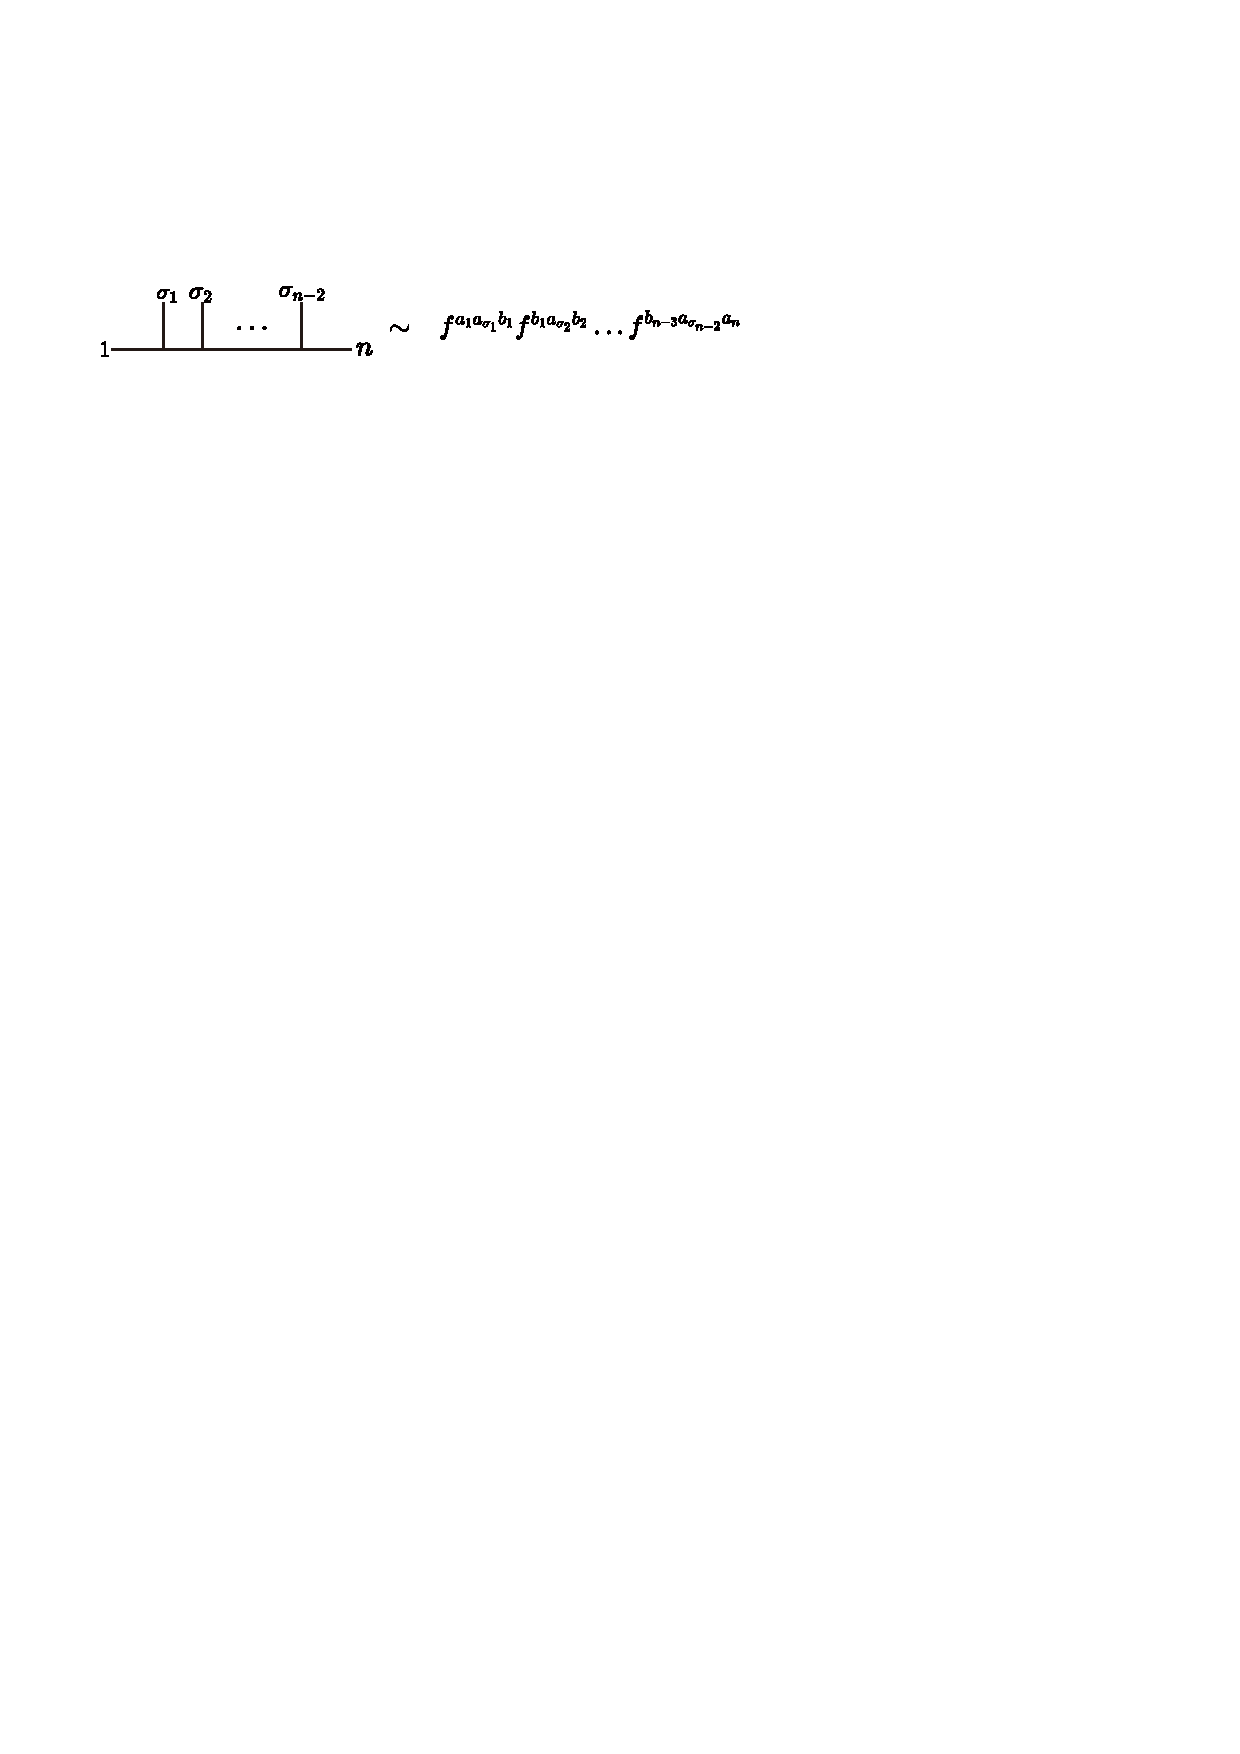
\includegraphics[width=0.95\linewidth]{figs/fig10.pdf}
	\caption{半梯子图}
	\label{fig:6.3}
\end{figure}

\begin{figure}[htbp]
	\centering
	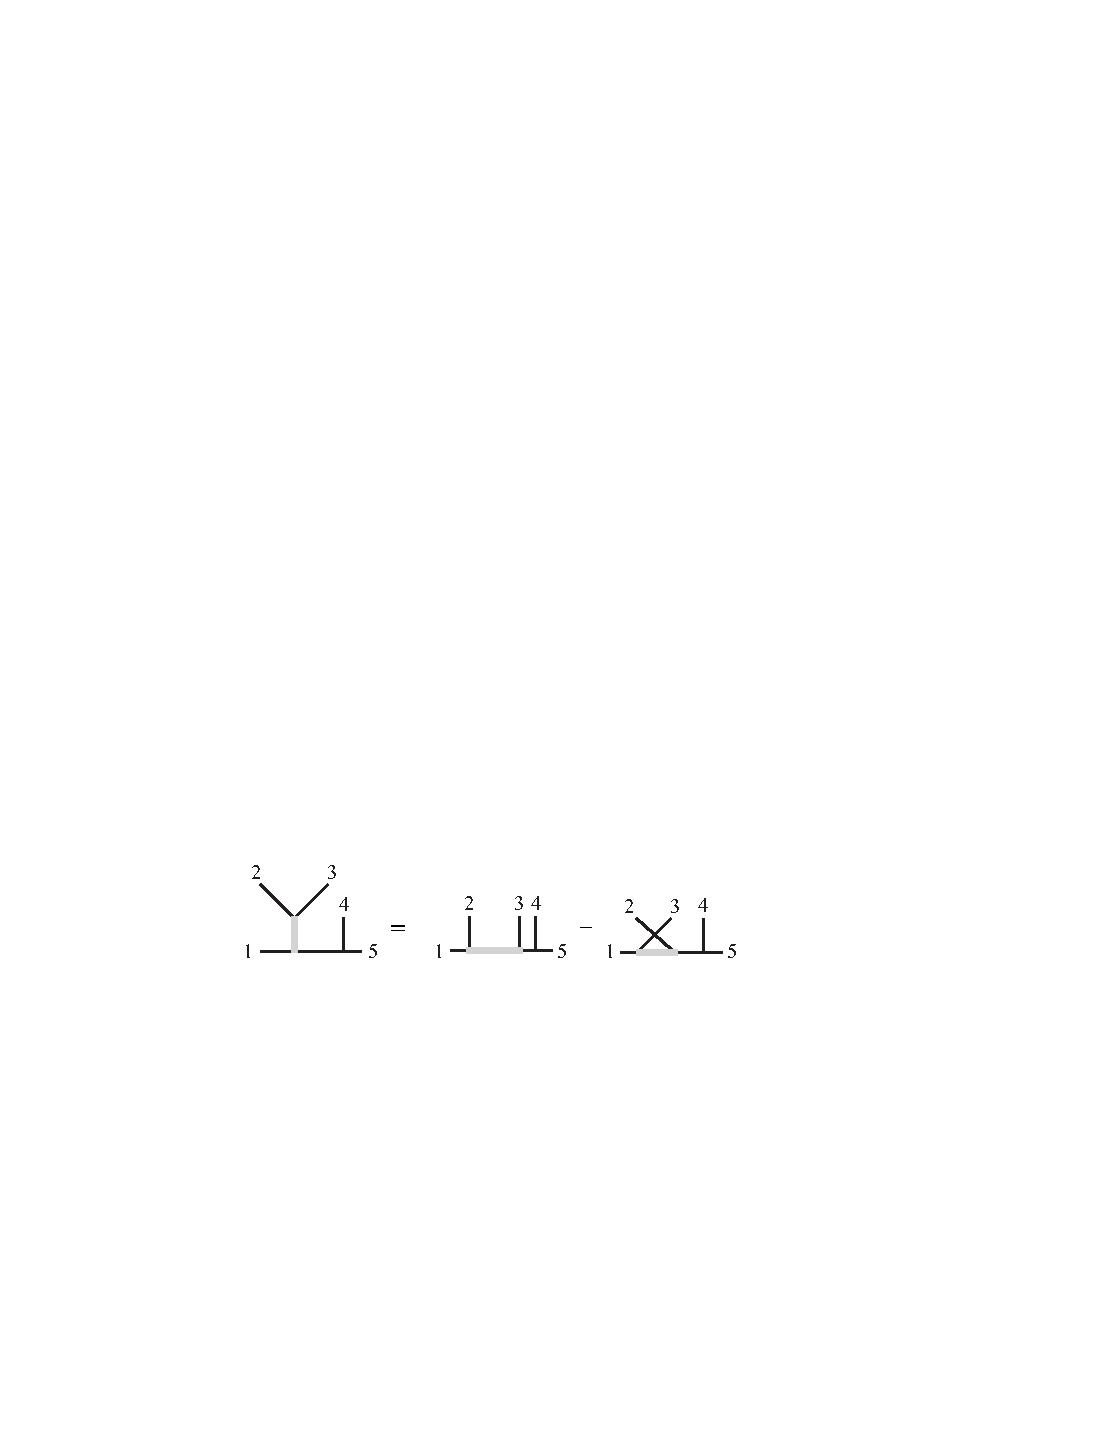
\includegraphics[width=0.90\linewidth]{figs/fig11.pdf}
	\caption{利用Jacobi恒等式转换到半梯子图}
	\label{fig:6.4}
\end{figure}

\begin{figure}[htbp]
	\centering
	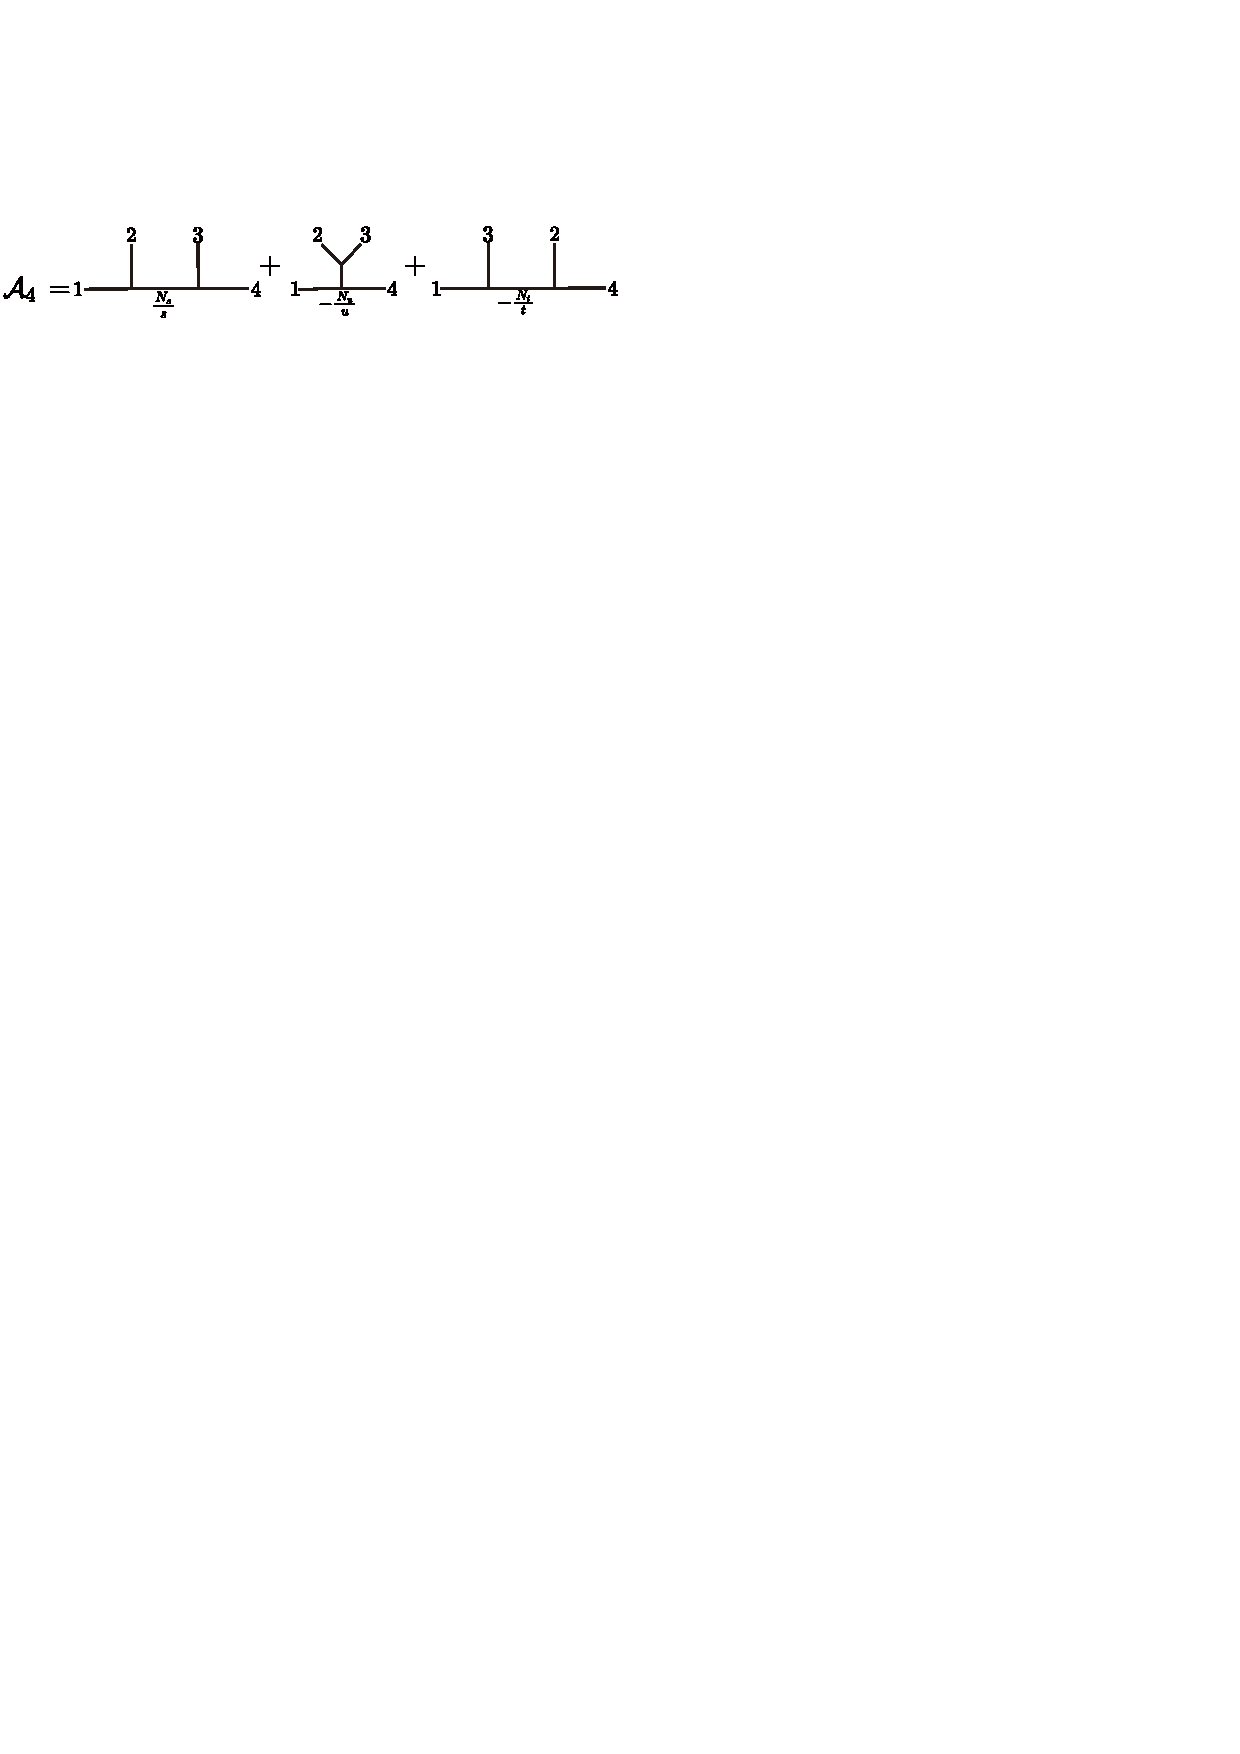
\includegraphics[width=0.90\linewidth]{figs/fig12.pdf}
	\caption{$\Gamma_4$的三幅图}
	\label{fig:6.5}
\end{figure}
比如四点Yang-Mills理论振幅有\ref{fig:6.5}三幅三顶角图有贡献。这里选取正负号约定是为了让$N_s+N_u+N_t=0$,对于树图$m$点情况$|\Gamma_m|=(2m-5)!!$。四点情况下只有两个偏振幅在Jacobi等式的意义下线性独立\footnote{当然如果加入BCJ恒等式两者也线性相关。},选取固定$1$和$4$。将\ref{fig:6.5}中第二个图利用Jacobi恒等式展开到半梯子图得到:
\begin{equation}
	A(1234) = \frac{N_s}{s}-\frac{N_u}{u},\quad A_4(1324)=-\frac{N_t}{t}+\frac{N_u}{u}
\end{equation}
不难看出上面偏振幅在\ref{eq:6.5}的变换下是规范不变的,其实就是在说单个三顶角图不是可观测量,但组合在一起得到的偏振幅规范不变。而且从$N_s+N_t+N_u=0$导出他们满足BCJ恒等式$sA_4(1,2,3,4)=tA_4(1,3,2,4)$。注意,如果$\{N_i\}$是BCJ分子,那么BCJ恒等式自然被满足,但BCJ恒等式本身是和\ref{eq:6.1}的参数化选取无关的,也就是说不管$\{N_i\}$如何选取,最终的振幅之间都满足BCJ恒等式。选取$N_s$和$N_u$为独立变量:
\begin{equation}
	\begin{pmatrix}A_4(1234)\\A_4(1324)\end{pmatrix}=\begin{pmatrix}\frac{1}{s}&-\frac{1}{u}\\\frac{1}{t}&\frac{1}{u}+\frac{1}{t}\end{pmatrix}\begin{pmatrix}N_s\\N_u\end{pmatrix}
\end{equation}
但是由于偏振幅之间满足BCJ恒等式,他们之间不是线性无关的,所以上面的矩阵其实不可逆。而这又恰恰说明了BCJ分子的不唯一性。

上面说的这些都仅仅只是色-运动学之间代数结构上的对偶,而这种对偶和规范理论与微扰引力理论振幅之间又密切关系。进一步有猜想,如果找到了一组BCJ分子,那么引力振幅可以直接由\ref{eq:6.1}得到:
\begin{equation}
	\mathcal{M}_n=\sum_{i\in\Gamma_n}\frac{N_iN_i}{D_i}=\sum_{i\in\Gamma_n}\frac{N_i\tilde{N}_i}{D_i}
\end{equation}
此式称为BCJ双复制关系。第二个等号是说明双复制的$n_i$可以只有一个是BCJ分子,另外一个可以不满足色运动学对偶,但是最终得到的振幅依然相同。利用半梯子图基底可以写成下式:
\begin{equation}
	\label{eq:6.14}
	M_n=\sum_{\sigma\in S_{n-2}}n_{1|\sigma_1,\sigma_2,\ldots,\sigma_{n-2}|n}A_n(1,\sigma_1,\sigma_2,\ldots,\sigma_{n-2},n)
\end{equation}
所以只需要知道半梯子图的BCJ分子就够了。前面我们讲过KLT关系,也是双复制的形式。实际上KLT关系可以看作是树图的一组特殊的BCJ双复制关系,可以从KLT关系直接构造出半梯子图的BCJ分子从而用Jacobi恒等式得到三顶点图的全部BCJ分子,比如四点五点KLT关系为:
\begin{equation}
\begin{aligned}
	M_4(1234)&=-s_{12}A_4(1234)A_4(1243),\\M_5(12345)&=s_{23}s_{45}A_5(12345)A_5(13254)+(3\leftrightarrow4)
\end{aligned}
\end{equation}
与\ref{eq:6.14}对照可以得到BCJ分子:
\begin{equation}
	\begin{aligned}
		n=4:\quad & n_{12,34} = -s_{12}\,A^{\text{tree}}_{4}[1243], \quad n_{13,24} = 0; \\
		n=5:\quad & n_{12,3,45} = s_{23}\,s_{45}\,A^{\text{tree}}_{5}[13254], \quad n_{12,4,35} = s_{24}\,s_{35}\,A^{\text{tree}}_{5}[14253]; \\
		& n_{13,4,25} = n_{14,2,35} = n_{14,3,215} = n_{12,3,415} = 0.
	\end{aligned}
\end{equation}
树图的BCJ双复制关系已经得到证明\cite{Bern:2010yg},但目前对于圈图BCJ分子的构造仍是一个未解之谜,不过已经构造出了不少例子\cite{Bern:2010ue,Bern:2012uf},这也让我们相信色-运动学对偶猜想的正确性。近年来,双复制关系也被用在引力波求解等问题上,详见综述\cite{Bern:2019prr,Adamo:2022dcm,Bern:2022wqg}。

\section{SYM振幅的超旋量空间表述}

\section{超弦无质量态$n$点盘面振幅}

\section{利用纯旋量超弦构造Yang-Mills理论的树图BCJ分子}